%--------------------------------------------------------------
% thesis.tex 
%--------------------------------------------------------------
% Corso di Laurea in Informatica 
% - template for the main file of Informatica@Unifi Thesis 
% - based on Classic Thesis Style Copyright (C) 2008 
%   Andr\'e Miede http://www.miede.de   
%--------------------------------------------------------------
\documentclass[twoside,openright,titlepage,fleqn,
	headinclude,12pt,a4paper,BCOR=5mm,footinclude]{scrbook}

\usepackage[nottoc]{tocbibind}
%--------------------------------------------------------------
% Inputs for the title page 
%--------------------------------------------------------------
\newcommand{\myItalianTitle}{Titolo italiano\xspace}
\newcommand{\myEnglishTitle}{English title\xspace}
% use the right myDegree option
\newcommand{\myDegree}{Corso di Laurea in Informatica\xspace}
%\newcommand{\myDegree}{Corso di Laurea Magistrale in Informatica\xspace}
\newcommand{\myName}{Candidate's Name Surname\xspace}
\newcommand{\mySupervisorTitle}{Relatore/Relatrice\xspace} %%% remove one of the two
\newcommand{\mySupervisorName}{\textit{Supervisor's Name Surname}\xspace} 
\newcommand{\myCoSupervisorTitle}{Correlatore/Correlatrice\xspace} %%% optional: remove this command if the thesis has no Co-Supervisor
\newcommand{\myCoSupervisorName}{\textit{Co-Supervisor's Name Surname}\xspace} %%% optional: remove this command if the thesis has no Co-Supervisor
\newcommand{\myTime}{Anno Accademico 202X-202Y\xspace}
%--------------------------------------------------------------


\usepackage{minted}

\usepackage[utf8]{inputenc} 
\usepackage[T1]{fontenc} 

% switch italian and english, depending on the language of the thesis
% this will change the chapter titles
%\usepackage[italian]{babel}
\usepackage[english]{babel}
\usepackage{csquotes}
\usepackage{comment}
\usepackage[fleqn]{amsmath}  
\usepackage{ellipsis}
\usepackage{listings}
\usepackage{subfig}
\usepackage{caption}
\usepackage{appendix}
\usepackage{siunitx}
\usepackage[pdftex]{graphicx} 
\graphicspath{{./Figures/}}
 \usepackage[eulerchapternumbers,linedheaders,subfig,beramono,eulermath,
parts,dottedtoc]{classicthesis}

\captionsetup[listing]{name=Listato}
\captionsetup[figure]{name=Figura}
%--------------------------------------------------------------
% Layout setting
%--------------------------------------------------------------
\newlength{\abcd} 
\newcommand{\myfloatalign}{\centering} 
\setlength{\extrarowheight}{3pt} 
\captionsetup{format=hang,font=small}

\usepackage{geometry}
\geometry{
	a4paper,
	ignoremp,
	bindingoffset = 1cm, 
	textwidth     = 13.5cm,
	textheight    = 21.5cm,
	lmargin       = 3.5cm, 
	tmargin       = 4cm    
}

\lstset{
  	frame=tb,
	language=Matlab,
  	aboveskip=3mm,
  	belowskip=3mm,
  	showstringspaces=false,
  	columns=flexible,
  	basicstyle={\small\ttfamily},
  	numbers=none,
  	breaklines=true,
  	breakatwhitespace=true,
  	tabsize=3
}

%--------------------------------------------------------------
\begin{document}
\frenchspacing
\raggedbottom
\pagenumbering{roman}
\pagestyle{plain}
%--------------------------------------------------------------
% Frontmatter
%--------------------------------------------------------------
\include{FrontMatter/Titlepage}
\pagestyle{scrheadings}
%--------------------------------------------------------------
% Mainmatter
%--------------------------------------------------------------
\pagenumbering{arabic}
\tableofcontents
\listoffigures
\cleardoublepage
\thispagestyle{empty}
\begin{flushright}
\null\vspace{\stretch {1}}
%--------------------------------------------------------------
% Citation
%--------------------------------------------------------------
\emph{"Se avessi avuto più tempo, avrei scritto una lettera più breve." \break --- Blaise Pascal} \vspace{\stretch{2}}\null
\end{flushright}
\cleardoublepage

%--------------------------------------------------------------
% Chapters
%--------------------------------------------------------------
% !TEX root = ../Thesis.tex

\chapter{Introduzione}
Negli ultimi anni, Rust è emerso come uno dei linguaggi di programmazione più promettenti e apprezzati dalla comunità degli sviluppatori, guadagnando popolarità in ambiti che richiedono elevate prestazioni e garanzie di sicurezza della memoria. Creato da Mozilla Research e successivamente adottato da grandi aziende come Microsoft, Google e Amazon, Rust offre un modello di gestione della memoria innovativo che elimina la necessità di un Garbage Collector, garantendo l'assenza di errori comuni come buffer overflow, dangling pointer e data race. Queste caratteristiche lo rendono particolarmente adatto per lo sviluppo di sistemi critici come sistemi operativi e infrastrutture di rete.

Tuttavia, Rust si discosta notevolmente dai linguaggi object-oriented tradizionali come Java, che da decenni domina lo sviluppo applicativo. Java, con la sua gestione automatica della memoria tramite Garbage Collector e il suo solido supporto al polimorfismo tramite ereditarietà e interfacce, ha semplificato lo sviluppo software per generazioni di programmatori. Il confronto tra questi due linguaggi non è solo accademico, ma ha implicazioni pratiche per sviluppatori che devono valutare quale tecnologia adottare.

Questa tesi si propone di analizzare sistematicamente le differenze fondamentali tra Rust e Java, concentrandosi su due aspetti chiave: la gestione della memoria e il supporto al polimorfismo. Attraverso un'analisi comparativa dei due aspetti, il lavoro mira a evidenziare le diverse scelte progettuali alla base di ciascun linguaggio e le loro implicazioni pratiche. 

Il metodo di analisi si basa sull'esame diretto delle caratteristiche linguistiche, supportato da esempi di codice comparativi che illustrano come concetti simili siano implementati in modo diverso nei due linguaggi. L'attenzione è rivolta non solo alle differenze sintattiche, ma anche alle implicazioni che ciascun approccio comporta sullo sviluppo del software.

La tesi è strutturata come segue: 
\begin{itemize}
    \item Capitolo 2: Panoramica dei tipi di dati nei due linguaggi, seguita dalla presentazione dei concetti fondamentali, come \texttt{struct} ed \texttt{enum} in Rust, necessari per la corretta comprensione dei capitoli successivi. 
    \item Capitolo 3: Analisi delle differenze nella gestione della memoria tra Rust e Java, con particolare attenzione ai concetti di ownership e borrowing in Rust, confrontati con il modello di Garbage Collection di Java.
    \item Capitolo 4: Analisi delle differenze nel supporto al polimorfismo, esaminando i meccanismi statici e dinamici offerti da entrambi i linguaggi. Il capitolo si conclude con una sezione che mostra, mediante un esempio pratico, come sia possibile estendere il comportamento nei due linguaggi sfruttando i rispettivi meccanismi di polimorfismo.
    \item Capitolo 5: In quest'ultimo capitolo vengono riassunti i principali risultati dell'analisi comparativa, evidenziando i punti di forza e le limitazioni di ciascun linguaggio nei due ambiti considerati. 
\end{itemize}

% !TEX root = ../Thesis.tex

\chapter{Concetti fondamentali}
In questo capitolo vengono introdotti i concetti fondamentali per la comprensione del lavoro svolto in questa tesi. In particolare, verrà fornita una panoramica sui tipi e sulla sintassi fondamentale di Rust, eseguendo un confronto con Java. 
\section{Tipi}
Sia Java che Rust sono linguaggi \textit{statically typed} (staticamente tipati), il che significa che ogni variabile ha un tipo conosciuto a compile time. Inoltre, sono anche \textit{strongly typed} (fortemente tipati), ossia che il type system del linguaggio applica rigorosamente regole di tipo, impedendo operazioni tra tipi incompatibili e limitando le operazioni che possono essere eseguite su un dato tipo. Questi concetti sono fondamentali per prevenire errori di tipo a runtime.

In Java sono presenti i seguenti tipi di tipi:
\begin{itemize}
    \item Tipi Primitivi: sono i tipi predefiniti dal linguaggio e includono:
        \begin{itemize}
            \item Tipi Numerici: \texttt{byte}, \texttt{short}, \texttt{int}, \texttt{long}, \texttt{char}, \texttt{float}, \texttt{double}. I primi cinque sono \textit{IntegralTypes} (interi), mentre gli ultimi due sono \textit{FloatingPointTypes} (virgola mobile).
            \item Tipo Booleano: \texttt{boolean}.
        \end{itemize} 
        Variabili di tipi primitivi contengono direttamente i valori e non possono essere \texttt{null}.
    \item Tipi Riferimento: sono memorizzati come riferimenti a oggetti nell' heap. Includono quattro diversi tipi di tipo riferimento:
        \begin{itemize}
            \item Tipo Classe.
            \item Tipo Interfaccia.
            \item Variabili di tipo: parametro di tipo utilizzato nella programmazione generica. 
            \item Tipo Array: definito utilizzando il nome di un tipo seguito dalle parentesi quadre \texttt{[]}. Ad esempio \texttt{int[]}, \texttt{String[]}.
        \end{itemize}
    \item Tipi parametrici: tipo Classe o Interfaccia nella forma \texttt{C<T1, T2, ..., Tn>}, dove \texttt{C} è il nome della classe o interfaccia e \texttt{T1, T2, ..., Tn} sono i parametri di tipo.
\end{itemize}
In Rust sono presenti i seguenti tipi di tipi:
\begin{itemize}
    \item Tipi primitivi:
        \begin{itemize}
            \item Tipo Booleano: \texttt{bool}.
            \item Tipi Numerici: \texttt{u8}, \texttt{u16}, \texttt{u32}, \texttt{u64}, \texttt{u128}, \texttt{i8}, \texttt{i16}, \texttt{i32}, \texttt{i64}, \texttt{i128}, \texttt{f32}, \texttt{f64}. I primi sei sono interi, mentre gli ultimi due sono virgola mobile.
            \item Tipo Testuale: \texttt{char} o \texttt{str}. 
            \item Tipo Never: \texttt{!}, rappresenta un tipo che non ha valori. Può essere utilizzato solo come tipo di ritorno di una funzione. Rappresenta il risultato di una computazione che non viene mai completata. 
        \end{itemize} 
    \item Tipi Sequenza: 
        \begin{itemize}
            \item Tipo Tupla: raggrupa insieme un insieme di valori di tipo diverso in un unico tipo composito. Ha dimensione fissa che equivale alla dimensione nel momento in cui viene dichiarata. Ad esempio, \texttt{(i32, f64, char)} è una tupla che contiene un intero a 32 bit, un numero in virgola mobile a 64 bit e un carattere.
            \item Tipo Array: tipo che rappresenta una collezione di elementi dello stesso tipo con una dimensione fissa. Ad esempio, \texttt{[i32; 5]} è un array di cinque interi a 32 bit.
            \item Tipo Slice: tipo che rappresenta una vista dinamica di una sequenza di elementi di tipo \texttt{T}. La sintassi è \texttt{[T]}. Solitamente viene utilizzata dietro a un tipo Puntatore.
        \end{itemize}
        \item Tipi definiti dall'utente: \texttt{struct}, \texttt{enum}, \texttt{union}. Trattati nel dettaglio nelle sezioni successive \ref{sec:structs} e \ref{sec:enums}.
        \item Tipi Funzione: tipi che rappresentano funzioni e chiusure (\textit{closure}). Una chiusura è una funzione anonima che può catturare variabili dall'ambiente circostante. La sintassi per definire una chiusura è \texttt{|parametri| espressione}.
        \item Tipi Puntatore: questo tipo comprende tre diversi tipi:
            \begin{enumerate}
                \item Tipo Riferimento: vedi sezione \ref{sec:borrowing}. 
                \item Tipo Raw Pointer: Per un tipo \texttt{T} si hanno \texttt{*const T} e \texttt{*mut T}. Sono puntatori senza garanzie di sicurezza e liveness.
                \item Tipo Smart Pointer: puntatori che forniscono funzionalità aggiuntive rispetto ai puntatori grezzi come la gestione automatica della memoria. I più comuni sono \texttt{Box<T>}, \texttt{Rc<T>} e \texttt{Arc<T>}. 
                \item Tipo Puntatore a funzione: dichiarati come \texttt{fn(\&T) -> U} per una funzione che prende un riferimento a \texttt{T} e restituisce un valore di tipo \texttt{U}.
            \end{enumerate}
        \item Tipi Trait (tratto, nel senso di caratteristica): 
        \begin{itemize}
            \item Tipi Trait Object (vedi sezione \ref{sec:trait_objects}).
            \item Tipi \texttt{impl Trait}: utilizzati in posizione di ritorno o come parametro di funzione per indicare che la funzione restituisce o accetta un tipo che implementa un certo trait. È una forma alternativa per indicare un tipo generico con un vincolo di trait (vedi sezione \ref{sec:rust_traits}).
        \end{itemize}
\end{itemize}
\section{Struct}
\label{sec:structs}
Una \texttt{struct} in Rust è un tipo di dato definito dall'utente che consente di raggruppare insieme più valori correlati in un'unica entità. In particolare, i valori all'interno di una struct possono essere di tipi diversi e, insieme al nome associato al valore, sono chiamati \textit{campi}. Per definire una struct si utilizza la keyword \texttt{struct} come segue:
\begin{minted}[fontsize=\small]{Rust}
    struct Book {
        title: String,
        pages: u32,
    }
\end{minted}
Per ottenere un comportamento analogo in Java si definisce una classe nel seguente modo:
\begin{minted}[fontsize=\small]{Java}
    class Book {
        String title;
        int pages;
    }
\end{minted}
Come una struct Rust, una classe Java definisce un tipo di dato che può contenere più valori di tipo diverso, chiamati \textit{campi}. Una struct può essere vista come una versione più leggera di una classe Java, in quanto non supporta l'ereditarietà e non può avere metodi direttamente associati ad essa (i metodi sono definiti separatamente in un blocco \texttt{impl}, come descritto più avanti).

Per creare un'istanza di una struct, si utilizza la seguente sintassi:
\begin{minted}[fontsize=\small]{Rust}
    let lotr = Book { 
        title: String::from("Il Signore degli Anelli"), 
        pages: 1216 
    };
\end{minted}
In Rust, il costruttore è implicito e si basa sulla sintassi di inizializzazione dei campi. In Java, invece, è necessario definire un costruttore esplicitamente come un metodo d'istanza all'interno della classe:
\begin{minted}[fontsize=\small]{Java}
    class Book {
        String title;
        int pages;

        // Costruttore
        public Book(String title, int pages) {
            this.title = title;
            this.pages = pages;
        }
    }
\end{minted}
Per creare un'istanza della classe si utilizza la keyword \texttt{new}:
\begin{minted}[fontsize=\small]{Java}
    Book lotr = new Book("Il Signore degli Anelli", 1216);
\end{minted}
In particolare, Rust non supporta l'inizializzazione di default dei campi di una struct, quindi è necessario fornire un valore per ogni campo al momento della creazione dell'istanza. Ad esempio:
\begin{minted}[fontsize=\small]{Rust}
    let hp = Book { 
        title: String::from("Harry Potter")
    };
\end{minted}
Questo codice genererebbe un errore di compilazione poiché il campo \texttt{pages} non è stato inizializzato. In Java, invece, se non si fornisce un valore per un campo, esso viene inizializzato con un valore di default (ad esempio, 0 per i tipi numerici e \texttt{null} per i tipi riferimento). Quindi il seguente codice Java sarebbe valido:
\begin{minted}[fontsize=\small]{Java}
    // assumendo che esista un costruttore 
    // public Book(String title)
    Book book2 = new Book("Harry Potter");
\end{minted}
In particolare, poiché Java supporta l'overloading, si possono avere costruttori in overload consentendo l'instanziazione di un oggetto in più modi. Questo è permesso anche grazie alla semantica di auto inizializzazione di Java. In generale, possiamo dire che l'approccio di Rust è molto più rigoroso e sicuro, infatti l'approccio Java può portare a errori di runtime se non si presta attenzione a come vengono inizializzati i campi.

Per accedere ai campi di una struct, e quindi potenzialmente cambiarne lo stato, si utilizza la notazione puntata come segue:
\begin{minted}[fontsize=\small]{Rust}
    let lotr_title = lotr.title; 
    let lotr_pages = lotr.pages;
\end{minted}
Da osservare che le variabili in Rust sono immutabili di default, quindi per modificare un campo di una variabile è necessario dichiarare la variabile come mutabile utilizzando la parola chiave \texttt{mut}:
\begin{minted}[fontsize=\small]{Rust}
    let mut lotr = Book { 
        title: String::from("Il Signore degli Anelli"), 
        pages: 1216 
    };
    lotr.pages = 1300; 
\end{minted}
In Java, la modifica del valore di una variabile d'istanza di una classe avviene in modo simile, tramite notazione puntata, a patto che chi modifica lo stato dell'oggetto sia autorizzato a farlo: ad esempio il campo è dichiarato \texttt{public} (e non \texttt{final}) oppure viene fornito un metodo della classe che consente di modificare il campo.

Nel lavoro svolto in questa tesi, si fa anche ampio utilizzo delle \textit{Unit-Like Structs}: strutture che non hanno campi ma possono essere utili quando si desidera definire un tipo che rappresenta un concetto o un'entità senza la necessità di memorizzare dati specifici. Un esempio di utilizzo di una unit-like struct è il seguente:
\begin{minted}[fontsize=\small]{Rust}
    struct MyStruct;

    // Per istanziare una unit-like struct
    // non sono necessarie parentesi graffe
    let instance = MyStruct;
\end{minted}
\subsection{Funzioni e metodi}
In Rust, una funzione si definisce con la parola chiave \texttt{fn}, seguita dal nome, da una lista di parametri racchiusi tra parentesi tonde e, se presente, dal tipo di ritorno. Ad esempio:
\begin{minted}[fontsize=\small]{Rust}
    fn add(a: i32, b: i32) -> i32 {
        a + b 
        // L'ultima espressione senza punto 
        // e virgola è il valore di ritorno
    }
    let result = add(5, 10); // Chiamata della funzione
    println!("Result: {}", result); // Stampa: Result: 15
\end{minted}
La funzione \texttt{add()} prende due parametri di tipo \texttt{i32} e restituisce la loro somma, anch'essa di tipo \texttt{i32}. Il tipo di ritorno è specificato dopo la freccia \texttt{->}.

Così come possiamo definire funzioni ``libere'', è possibile associare funzioni a una \texttt{struct} (o un \texttt{enum} come vedremo nella prossima sezione) tramite l'uso di un blocco \texttt{impl}. Queste funzioni prendono il nome di \textit{funzioni associate} poiché sono legate a una specifica struct. Le funzioni associate che prendono come primo parametro \texttt{self} sono chiamate \textit{metodi} e possono essere chiamati tramite notazione puntata. \texttt{Self} è una keyword Rust che rappresenta l'istanza della struct su cui il metodo viene chiamato. Ad esempio, per la struct \texttt{Book} definita in precedenza, un blocco \texttt{impl} potrebbe apparire come nel listato \ref{lst:method_example}.
\begin{listing}
    \begin{minted}[fontsize=\small]{Rust}
    impl Book {
        fn describe(&self) {
            println!("\"{}\" has {} pages.", self.title, self.pages);
        }

        fn is_long(&self) -> bool {
            self.pages > 300
        }
    }

    fn main() {
        let lotr = Book { 
            title: String::from("Il Signore degli Anelli"),
            pages: 1216
        };
        lotr.describe(); // Chiamata del metodo
    }
    \end{minted}
    \caption{Esempio di metodo in Rust.}
    \label{lst:method_example}
\end{listing}

Il parametro \texttt{self} può essere passato in diversi modi, a seconda di come si desidera utilizzare l'istanza della struct all'interno del metodo, spesso è passato tramite riferimento per motivi di ownership e borrowing (vedi sezione \ref{sec:borrowing}). In Java, esiste un concetto simile a \texttt{self} che è \texttt{this}: un riferimento implicito all'istanza corrente della classe. A differenza di \texttt{self}, \texttt{this} è sempre disponibile e non è necessario dichiararlo esplicitamente. In generale, i metodi di una struct definiscono il comportamento associato a un'istanza di quella struct.

Invece, le funzioni associate che non prendono \texttt{self} come primo parametro sono spesso usate come costruttori o funzioni di utilità legate alla struct ma non a una specifica istanza. Ad esempio:
\begin{listing}[H]
    \begin{minted}[fontsize=\small]{Rust}
        impl Book {
            fn new(title: String, pages: u32) -> Self {
                Self { title, pages }
            }
        }
    \end{minted}
    \caption{Esempio di funzione associata in Rust.}
    \label{lst:associated_function_example}
\end{listing}
\texttt{Self} in posizione di tipo di ritorno di una funzione associata si riferisce al tipo della struct stessa, in questo caso \texttt{Point}. Per chiamare questo tipo di funzioni associate, si utilizza la sintassi \texttt{NomeStruct::nome\_funzione()}:
\begin{minted}[fontsize=\small]{Rust}
    let book = Book::new(String::from("1984"), 328);
\end{minted}
In particolare, nel listato \ref{lst:associated_function_example}, si è utilizzato un forma più breve e leggera per inizializzare i campi della struct. Questa sintassi è utilizzata quando i nomi dei parametri della funzione corrispondono ai nomi dei campi della struct. In questo caso, \texttt{Self \{ title, pages \}} è equivalente a \texttt{Self \{ title: title, pages: pages \}}. Java non mette a disposizione questo tipo di funzionalità, anzi in Java lo sviluppatore è tenuto a disambiguare esplicitamente i nomi dei parametri del costruttore dai nomi delle variabili d'istanza della classe utilizzando la parola chiave \texttt{this}.

In Java, il concetto di funzione associata è superfluo poiché le funzioni sono sempre definite, e quindi associate, all'interno di una classe. I metodi Rust sono analoghi ai metodi di istanza in Java, ossia metodi che appartengono a un'istanza specifica di una classe. Quindi, il listato \ref{lst:method_example} potrebbe essere tradotto in Java con il codice riportato nel listato \ref{lst:java_method_example}.
\begin{listing}
\begin{minted}[fontsize=\small]{Java}
    class Book {
        
        ...

        public void describe() {
            System.out.println("\"" 
                               + title 
                               + "\" has " 
                               + pages 
                               + " pages.");
        }

        public boolean isLong() {
            return pages > 300;
        }
    }

    public class Main {
        public static void main(String[] args) {
            Book lotr = new Book("Il Signore degli Anelli", 1216);
            lotr.describe(); // Chiamata del metodo
        }
    }
\end{minted}
    \caption{Listato \ref{lst:method_example} in Java.}
    \label{lst:java_method_example}
\end{listing}

Invece, le funzioni ``libere'' in Java sono implementate come metodi statici. I metodi statici appartengono alla classe stessa piuttosto che a un'istanza specifica della classe. Questi sono spesso utilizzati come costruttori alternativi, come è il caso del pattern creazionale \textit{Static Factory Methods} \cite{gamma-design-patterns}, o per definire funzioni di utilità che non richiedono l'accesso ai dati di un'istanza specifica della classe. 
\section{Enum}
\label{sec:enums}
Un \texttt{enum} in Rust è un tipo di dato definito dall'utente che consente di rappresentare una variabile che può assumere uno tra un insieme finito di valori, chiamati \textit{varianti}. Un enum Rust è dichiarato utilizzando la parola chiave \texttt{enum} come segue:
\begin{minted}[fontsize=\small]{Rust}
    enum Shape {
        Circle,
        Rectangle,
        Triangle,
        Point,  
    }
\end{minted}
In Java, un enum è dichiarato in maniera analoga:
\begin{minted}[fontsize=\small]{Java}
    enum Shape {
        CIRCLE,
        RECTANGLE,
        TRIANGLE,
        POINT; 
    }
\end{minted}
In entrambi i linguaggi è possibile associare dati alle varianti di un enum. Tuttavia, c'è una differenza sostanziale tra la flessibilità con cui si può eseguire questa associazione.
\begin{itemize}
    \item In Java, un enum è classe speciale in cui le varianti sono istanze singleton statiche e finali di quella classe. Questo significa che ogni variante deve essere inizializzata esplicitamente nel momento della sua dichiarazione o all'interno di un blocco \texttt{static {}}. Ad esempio, se volessimo associare un numero di lati a ogni variante dell'enum \texttt{Shape}, in Java potremmo farlo nel seguente modo:
\begin{minted}[fontsize=\small]{Java}
    enum Shape {
        CIRCLE(0), RECTANGLE(4), TRIANGLE(3), POINT(0);

        private int sides;

        private Shape(int sides) {
            this.sides = sides;
        }
    }
\end{minted}
    La limitazione di questo approccio è che tutte le varianti dell'enum devono avere lo stesso insieme di dati associati, il che può essere restrittivo in alcuni casi. Ad esempio, se volessimo associare dati diversi a ogni variante, come il raggio per il cerchio, la larghezza e l'altezza per il rettangolo, e i lati per il triangolo, non sarebbe possibile farlo direttamente con gli enum di Java.

    Inoltre, il valore associato a una variante di un enum in Java è immutabile, quindi non può essere cambiato dopo l'inizializzazione, che avviene nel momento della dichiarazione.
    \item Rust, invece, consente di associare dati diversi, sia in tipo che in numero, a ogni variante, rendendo gli enum Rust molto più flessibili e potenti. Ad esempio, questo codice è possibile in Rust:
\begin{listing}[H]
    \begin{minted}[fontsize=\small]{Rust}
        enum Shape {
            Circle(f64),               // raggio
            Rectangle(f64, f64),      // larghezza, altezza
            Triangle(f64, f64, f64),  // lati
            Point,  
        }
    \end{minted}
    \caption{Esempio di enum in Rust con varianti che contengono dati.}
    \label{lst:enum_example}
\end{listing}
    In particolare, l'esempio sopra può essere reso più chiaro utilizzando nomi per i campi tramite la seguente sintassi:
\begin{minted}[fontsize=\small]{Rust}
    enum Shape {
        Circle { radius: f64 },
        Rectangle { width: f64, height: f64 },
        Triangle { a: f64, b: f64, c: f64 },
        Point,  
    }
\end{minted}
Inoltre, a differenza di Java, è possibile definire il valore dei dati associati a una variante nel momento della sua istanziazione:
\begin{minted}[fontsize=\small]{Rust}
    let circle = Shape::Circle { radius: 5.0 };
\end{minted}
\end{itemize}  
Un'altra differenza molto importante tra gli enum di Java e Rust è il modo in cui si esegue il pattern matching sulle varianti. Per pattern matching si intende la capacità di verificare quale variante di un enum è attualmente in uso e di estrarre i dati associati a quella variante. In Rust, il pattern matching è eseguito tramite la parola chiave \texttt{match}. Ad esempio, considerando il listato \ref{lst:enum_example}, si potrebbe scrivere una funzione per calcolare l'area di una figura geometrica come segue:
\begin{minted}[fontsize=\small]{Rust}
    fn area(shape: &Shape) -> f64 {
        match shape {
            Shape::Circle(radius) => 3.14 * radius * radius,
            Shape::Rectangle(width, height) => width * height,
            Shape::Triangle(a, b, c) => {
                // Compute area for triangle
            }
            Shape::Point => 0.0,
        }
    }
\end{minted}
In particolare, in Rust, il pattern matching è esaustivo, ossia il compilatore verifica che tutti i casi possibili siano coperti, garantendo così la sicurezza del codice. Ad esempio:
\begin{minted}[fontsize=\small]{Rust}
    fn area(shape: &Shape) -> f64 {
        match shape {
            Shape::Circle(radius) => 3.14 * radius * radius,
            Shape::Rectangle(width, height) => width * height,
            Shape::Point => 0.0,
        }
    }
    // Questo codice non compila perché manca il caso per Triangle
\end{minted}
In Java, il pattern matching sugli enum è meno potente e richiede l'uso di costrutti come \texttt{switch}. A differenza di Rust, Java non garantisce che tutti i casi siano coperti, il che può portare a errori di runtime se una variante non viene gestita. Ad esempio:
\begin{minted}[fontsize=\small]{Java}
    enum Status {
        SUCCESS,
        FAILURE,
        PENDING
    }

    public String getStatusMessage(Status status) {
        switch (status) {
            case SUCCESS:
                return "Operation was successful.";
            case FAILURE:
                return "Operation failed.";
            // Manca il caso per PENDING
            default:
                return "Unknown status.";
        }
    }
\end{minted}
Questo codice compila, ma se venisse passato il valore \texttt{PENDING} si verificherebbe un comportamento inatteso: il messaggio di stato restituito sarà \texttt{"Unknown status."}, anche se lo stato in realtà è noto. Inoltre, in Java non è possibile estrarre dati associati a una variante di un enum all'interno di un costrutto \texttt{switch}, a meno di definire metodi aggiuntivi all'interno dell'\texttt{enum}. 

Quindi, si può notare come gli enum di Rust offrano funzionalità molto più potenti e flessibili: è possibile associare dati diversi a ciascuna variante e accedervi direttamente durante il pattern matching. Per ottenere un comportamento simile in Java, sarebbe necessario ricorrere a soluzioni più complesse, ad esempio usando interfacce \texttt{sealed} e \texttt{record}:
\begin{minted}[fontsize = \small]{Java}
    sealed interface Shape permits Circle, Rectangle, Triangle, Point {}

    record Circle(double radius) implements Shape {}
    record Rectangle(double width, double height) implements Shape {}
    record Triangle(double a, double b, double c) implements Shape {}
    record Point() implements Shape {}

    public double area(Shape shape) {
        return switch (shape) {
            case Circle c -> 3.14 * c.radius() * c.radius();
            case Rectangle r -> r.width() * r.height();
            case Triangle t -> {
                // Compute area for triangle
            }
            case Point p -> 0.0;
        };
    }
\end{minted}
In questo esempio, si definisce un'interfaccia \texttt{Shape} che è \texttt{sealed}, il che significa che solo le classi specificate (in questo caso, i record) possono implementarla. Ogni ``variante'' è rappresentata come un \texttt{record} che implementa l'interfaccia \texttt{Shape}. Il pattern matching viene eseguito utilizzando un costrutto \texttt{switch} che è in grado di estrarre i dati associati a ciascun record. Tuttavia, questo approccio è più verboso e complesso rispetto alla semplice definizione di un enum in Rust. Tuttavia, in questo caso, Java garantisce l'esaustività del pattern matching grazie all'uso di interfacce \texttt{sealed}.

Infine, analogamente a quello che succede per le struct, anche gli enum in Rust possono avere metodi associati definiti all'interno di un blocco \texttt{impl}. Ad esempio:
\begin{minted}[fontsize=\small]{Rust}
    impl Shape {
        fn area(&self) -> f64 {
            match self {
                /* ... */
            }
        }
    }

    fn main() {
        let circle = Shape::Circle { radius: 5.0 };
        println!("Area: {}", circle.area());
    }
\end{minted}
In Java, i metodi associati a un enum sono definiti all'interno della dichiarazione dell'enum stesso come avviene per una qualsiasi classe.
% !TEX root = ../Thesis.tex

\chapter{Gestione della memoria}

\section{L'approccio di Java}
Java è un linguaggio di programmazione progettato per essere semplice da usare e portabile, con una gestione della memoria che mira a garantire sicurezza e facilità d'uso a scapito di un controllo diretto da parte del programmatore. Java raggiunge questi obiettivi principalmente attraverso l'uso di un \textit{garbage collector} e un ambiente di esecuzione controllato (la Java Virtual Machine - JVM). Gli aspetti fondamentali dell'approccio di Java sono:

\begin{enumerate}
\item La gestione automatica della memoria tramite il garbage collector, che si occupa di identificare e liberare la memoria occupata da oggetti non più raggiungibili nel programma, prevenendo così problemi comuni, come i memory leak. Questo, di fatto, toglie al programmatore la responsabilità collegata al dover gestire manualmente l'allocazione e la deallocazione della memoria, riducendo la probabilità di errori nel codice.
\item La prevenzione di comportamenti indefiniti principalmente a run-time, attraverso un controllo rigoroso dell'accesso alla memoria e la gestione delle eccezioni. 
\end{enumerate}

Sebbene l'approccio di Java renda lo sviluppo più semplice e sicuro rispetto a linguaggi senza garbage collector, come C e C++, l'uso del garbage collector introduce una certa imprevedibilità nelle prestazioni, in quanto il processo di garbage collection deve essere eseguito in concorrenza con l'esecuzione del programma. 
\section{L'approccio di Rust}
Rust è un linguaggio di programmazione che si distingue per la sua gestione della memoria, evitando la necessità di un garbage collector e garantendo al contempo sicurezza e prestazioni elevate. Rust ha due obiettivi principali:
\begin{enumerate}
    \item  Garantire che il programma sia privo di comportamenti indefiniti, ovvero situazioni in cui il programma può agire in modo imprevedibile. Un esempio tipico è l'accesso a memoria non valida, che può portare all'esecuzione di codice con dati non inizializzati o causare errori di memoria come segmentation fault. 
    \item Prevenire comportamenti indefiniti a compile-time, piuttosto che a run-time. Questo significa che il compilatore di Rust è in grado di rilevare e segnalare errori di memoria prima che il programma venga eseguito, riducendo il rischio di bug e di errori durante l'esecuzione. Inoltre, viene ridotto il numero di controlli a run-time, migliorando le prestazioni del programma. 
    % Nell'articolo di google viene riportato il vantaggio di non avere controlli a run-time.
\end{enumerate}
Rust non può prevenire tutti i bug ma le metodologie messe in atto per la gestione della memoria rendono un programma scritto in Rust molto più sicuro rispetto a uno scritto in linguaggi con meno controlli. 

Un esempio concreto dell'efficacia di Rust nella prevenzione degli errori di memoria è fornito da Google \cite{android13-memorysafe}, che ha introdotto il linguaggio nello sviluppo di Android 13. In particolare, circa il 21\% del nuovo codice introdotto in Android 13 è stato scritto in Rust, e, alla data della pubblicazione dell'articolo, sono state scoperte zero vulnerabilità di sicurezza legate alla memoria in questo codice. Questo è un risultato significativo che dimostra come gli obiettivi prefissati da Rust siano stati raggiunti nella pratica.

Rust realizza questi obiettivi attraverso un sistema basato sui concetti di \textit{ownership} e \textit{borrowing}. Concetti fondamentali che verrano affrontati in dettaglio nelle prossime sezioni.

\section{Stack e Heap}
Sia Java che Rust utilizzano due aree di memoria principali: lo stack e l'heap, ma la loro gestione è profondamente diversa, riflettendo i diversi modelli di memoria adottati dai due linguaggi.

Lo stack è un'area di memoria strutturata con una struttura dati stack LIFO (Last In, First Out). La memoria stack è contigua e i dati memorizzati al suo interno sono in posizione fissa rispetto allo stack pointer, un puntatore che punta all'ultimo elemento inserito. Questo permette un accesso rapido ai dati usando indirizzi di memoria calcolati in modo semplice tramite un offset rispetto allo stack pointer. Inoltre, allocazione e deallocazione della memoria stack sono molto veloci poiché avvengono spostando lo stack pointer, avanti o indietro, di un numero di byte opportuno rispetto alla dimensione del dato e all'architettura della CPU.

L'heap, al contrario, è un'area di memoria non strutturata, in cui i dati possono essere allocati in qualsiasi sua posizione. L'allocazione e la deallocazione della memoria heap richiedono operazioni più complesse rispetto allo stack, poiché il sistema operativo deve tenere traccia degli spazi liberi e occupati. Questo può portare a un utilizzo meno efficiente della memoria (frammentazione) e a un accesso più lento ai dati rispetto allo stack. 

In Java, l'allocazione della memoria è fortemente automatizzata. Ogni volta viene creato un oggetto, tramite la keyword \texttt{new}, viene allocata memoria heap nel quale sarà memorizzato l'oggetto. L'uso dello stack è limitato a variabili di tipo primitivo e variabili locali. Al contrario, Rust adotta un modello più esplicito e flessibile. In rust, la variabili possono essere allocate sia nello stack che nell'heap, a seconda dalla conoscenza a compile time delle dimensioni del dato:
\begin{itemize}
    \item  Se la variabile ha una dimensione fissa nota a compile time, viene allocata nello stack. É possibile allocare nell'heap anche variabili di dimensione fissa attraverso \texttt{Box}.
    \item  Se la variabile ha una dimensione variabile o non nota a compile time, viene allocata nell'heap. 
\end{itemize} 
Questa è una differenza fondamentale rispetto a Java, perchè permette allo sviluppatore di avere più controllo su dove vengono allocati i dati, permettendo ottimizzazioni specifiche per le esigenze del programma. 

Ad esempio, sia in Java che in Rust, gli array hanno una dimensione fissa. Tuttavia, in Java, gli array sono allocati nell'heap e sono referenziati da variabili nello stack, mentre in Rust, poiché si conosce la loro dimensione a compile time, vengono allocati nello stack. Questo rende l'accesso agli elementi dell'array di Rust più veloce. 
\begin{minted} [fontsize=\small] {Java}
    int[] arr = {1, 2, 3, 4, 5}; // Array allocato nell'heap
    System.out.println("Il primo elemento e': " + arr[0]);
\end{minted}
\begin{minted} [fontsize=\small] {Rust}
    let arr = [1, 2, 3, 4, 5]; // Array allocato nello stack
    println!("Il primo elemento e': {}", arr[0]);
\end{minted}
\section{Ownership}
L'ownership è un concetto fondamentale in Rust il quale può essere definito come un insieme di regole che il compilatore controlla per garantire una corretta gestione della memoria. Questo significa sia garantire che non ci siano errori di memoria a run-time, sia che la memoria inutilizzata venga rilasciata correttamente per non terminare lo spazio di memoria disponibile (\textit{memory leak}). 

L'obiettivo principale dell'ownership è, quindi, quello di gestire la memoria heap tenendo traccia di quali parti di codice utilizzano valori contenuti in essa, minimizzare valori duplicati e garantire che la memoria venga rilasciata quando non è più necessaria. 
%TODO: Forse inserire confronto con Java su performance e garbage collector 

L'ownership si basa su tre regole principali: 
\begin{enumerate}
    \item  Ogni valore in Rust ha un \textit{owner}, ovvero una variabile che ne detiene la proprietà. 
    \item  Un valore può avere un solo owner alla volta. 
    \item  Quando l'owner di un valore esce dallo scope, il valore viene automaticamente rilasciato dalla memoria.
\end{enumerate}
Consideriamo un caso banale in cui si crea una variabile all'interno di uno scope:
\begin{minted} [fontsize=\small] {Rust}
    {
        let s = String::from("Hello");
    }
\end{minted}
In questo caso, secondo la regola 3, quando la variabile \texttt{s} esce dallo scope, il valore \texttt{"Hello"} viene automaticamente rilasciato dalla memoria. Questo avviene attraverso la funzione \texttt{drop} che viene chiamata automaticamente da rust quando la variabile va fuori dallo scope. In java questo non accade. Dato il seguente codice equivalente in Java:
\begin{minted} [fontsize=\small] {Java}
    {
        String s = "Hello";
    }
\end{minted}
La memoria occupata dalla stringa \texttt{"Hello"} non viene rilasciata automaticamente quando la variabile \texttt{s} esce dallo scope ma solo quando il garbage collector esegue la raccolta dei valori non più raggiungibili. Già da questo semplice caso si può notare come l'ownership di Rust permetta di avere un controllo più preciso sulla memoria. 

Un altro aspetto importante dell'ownership è che, quando si assegna un valore a un'altra variabile, l'ownership viene trasferita. Ad esempio, consideriamo il seguente codice:
\begin{minted} [fontsize=\small] {Rust}
    let s1 = String::from("Hello");
    let s2 = s1; // Ownership di s1 viene trasferita a s2
    // println!("{}", s1); // Errore di compilazione
    println!("{}", s2);
\end{minted}
In questo caso, l'ownership della stringa \texttt{"Hello"} viene trasferita da \texttt{s1} a \texttt{s2}. Dopo il trasferimento, \texttt{s1} non è più valida e qualsiasi tentativo di accedervi causerà un errore di compilazione. 
\begin{figure}[H]
    \label{fig:own1}
    \centering
    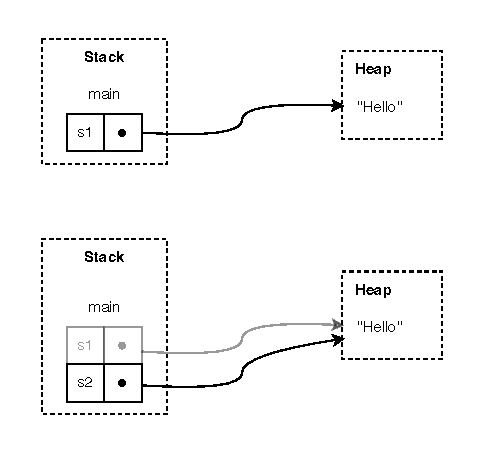
\includegraphics[scale = 1]{Figures/own1.pdf}
    \caption{Visualizzazione memoria Rust dopo il trasferimento di ownership.}
\end{figure}
In Rust, per variabili il cui valore è contenuto in memoria heap, un'istruzione di copia esegue una \textit{shallow copy} del valore e invalida la variabile originale. Questo comportamento prende il nome di \textit{move}. Rust non esegue mai una \textit{deep copy} di una variabile: se il programmatore desidera duplicare effettivamente il contenuto, deve farlo in modo esplicito (ad esempio usando il metodo \texttt{clone()}). Quindi, l'operazione di copia base è poco costosa in termini di performance.

Questo non è consistente con quello che accade in Java, dove l'assegnazione di un oggetto a un'altra variabile non invalida quella originale, ma crea una nuova referenza all'oggetto esistente. Entrambe le variabili possono accedere all'oggetto, condividendono lo stato. In Java, il codice equivalente sarebbe:
\begin{minted} [fontsize=\small] {Java}
    String s1 = "Hello";
    String s2 = s1; 
    System.out.println(s1); // Valido
    System.out.println(s2); // Valido
\end{minted}
In questo caso, quindi, entrambe le stringhe verrebbero correttamente stampate. L'approccio adottato da Rust è decisamente più restrittivo, ma si tratta di una caratteristica desiderabile: consente infatti di evitare errori comuni legati alla gestione della memoria, come l'accesso a variabili non più valide o la modifica involontaria di dati condivisi. 
Ad esempio, in Java, il codice seguente potrebbe causare un comportamento indesiderato:
\begin{minted} [fontsize=\small] {Java}
    class Person {
        String name;
        Person(String name) {
            this.name = name;
        }
    }

    public class Main {
        public static void main(String[] args) {
            Person p1 = new Person("Alice");
            Person p2 = p1; // p2 è una referenza a p1
            p2.name = "Bob"; // Modifica il nome di p1
            System.out.println(p1.name); // Stampa "Bob"
        }
    }
\end{minted}
In questo esempio, la modifica del campo \texttt{name} di \texttt{p2} influisce anche \texttt{p1}, poiché entrambi i riferimenti puntano allo stesso oggetto in memoria. Questo comportamento puà causare bug sottili e difficili da individuare, spcialmente in contesti complessi o concorrenti. In Rust, invece, il trasferimento di ownership impedisce il comportamento appena descritto, poiché una volta che l'ownership è stata trasferita, la variabile originale non può più essere utilizzata.
%TODO: dall'esempio precedente posso passare a rust con passaggio di parametro a funzione

% !TEX root = ../Thesis.tex

\chapter{Polimorfismo}
Il polimorfismo è un concetto fondamentale della programmazione. Derivato dal greco “molte forme”, il polimorfismo consente a entità di assumere diverse forme o comportamenti in base al contesto, permettendo di scrivere codice più flessibile, estendibile e manutenibile. Grazie al polimorfismo, è possibile utilizzare un'interfaccia comune per manipolare elementi di tipi diversi, facilitando così l'implementazione di soluzioni generiche. Il vantaggio principale del polimorfismo è il miglioramento della qualità del codice:
\begin{itemize}
    \item Favorisce l'astrazione, consentendo di trattare oggetti di tipi diversi in modo uniforme.
    \item Riduce la duplicazione di codice, poiché le operazioni comuni possono essere definite una sola volta e riutilizzate per diversi tipi.
    \item Semplifica la gestione delle estensioni future, poiché nuove funzionalità possono essere aggiunte senza modificare il codice esistente.
\end{itemize}
In un linguaggio come Java, orientato agli oggetti, il polimorfismo è una caratteristica centrale e largamente supportata tramite ereditarietà e interfacce. Rust, pur non essendo un linguaggio tradizionalmente orientato agli oggetti, offre un approccio alternativo al polimorfismo, basato su trait e tipi generici, che permette di ottenere astrazione e flessibilità.

In questo capitolo verrà fornita una panoramica delle modalità con cui Java e Rust implementano e sfruttano il polimorfismo, confrontando i due linguaggi.

\section{Polimorfismo in Java}
Java supporta il polimorfismo attraverso due principali meccanismi: il \textit{subtyping} (polimorfismo per inclusione) e il \textit{parametric polymorphism} (polimorfismo parametrico). 

Il subtyping si basa sul fatto che ci possa essere una relazione tra tipi chiamata \textit{relazione di sottotipo}. Si dice che un tipo \textit{A} è un sottotipo di un tipo \textit{B} quando il contesto richiede un elemento di tipo \textit{B} ma può accettare un elemento di tipo \textit{A}. In Java, la relazione di sottotipo viene implementata attraverso l'ereditarietà e le interfacce. Le classi possono estendere altre classi e implementare interfacce, consentendo agli oggetti di essere trattati come istanze della loro classe base o interfaccia. 

Il parametric polymorphism permette di assegnare a una parte di codice un tipo generico, utilizzando variabili di tipo al posto di tipi specifici, che poi possono essere istanziate con tipi concreti al momento dell'utilizzo.
\section{Polimorfismo in Rust}
In Rust, il polimorfismo è implementato attraverso i concetti di \textit{trait} e i \textit{generics}. I trait sono simili alle interfacce in Java e definiscono un insieme di metodi che un tipo deve implementare per essere considerato conforme a quel trait. I generics consentono di scrivere funzioni e strutture dati che possono operare su tipi diversi senza dover specificare un tipo concreto. Tramite l'uso dei generics si ottiene il \textit{parametric polymorphism}, come in Java, mentre attraverso i trait si ottiene il \textit{bounded parametric polymorphism}, che consente di specificare vincoli sui tipi generici.
\section{Generics: Monomorphization e Type Erasure}
\label{sec:generics}
Sia Rust che Java supportano la programmazione generica, che consente di scrivere codice che può operare su tipi diversi senza dover duplicare il codice per ogni tipo specifico. La sintassi per definire i generics in Rust e Java è simile, utilizzando parentesi angolare per specificare i parametri di tipo. Tuttavia, ci sono differenze significative nella gestione dei generics tra i due linguaggi.

Il compilatore Java utilizza un processo chiamato \textit{type erasure} per implementare i generics, questo include i seguenti fatti:
\begin{itemize}
    \item Durante la compilazione i parametri di tipo vengono sostituiti con il tipo \texttt{Object} o con un tipo specifico se è stato definito un vincolo sul parametro di tipo.
    \item Vengono inseriti cast espliciti per mantenere la type safety.
    \item Generazione di \textit{Bridge Methods} per preservare il polimorfismo dopo il processo di type erasure.
\end{itemize}
Ad esempio:
\begin{minted} [fontsize=\small] {Java}
    public class GenericClass<T> {
        T value;

        void setValue(T value) { 
            this.value = value;
        }
    }
\end{minted}
Dopo la type erasure, il codice diventa:
\begin{minted} [fontsize=\small] {Java}
    public class GenericClass {
        Object value;

        void setValue(Object value) { 
            this.value = value;
        }
    }
\end{minted}
Nel caso in cui, invece, si definisca un vincolo di tipo, ad esempio \texttt{<T extends Number>}, il compilatore Java sostituirà \texttt{T} con \texttt{Number} durante la type erasure, mantenendo la type safety:
\begin{minted} [fontsize=\small] {Java}
    public class GenericClass{
        Number value;

        void setValue(Number value) { 
            this.value = value;
        }
    }
\end{minted}
Quando si combina la type erasure con l'overriding dei metodi, Java genera dei \textit{Bridge Methods} per garantire che il polimorfismo funzioni correttamente. Uno scenario tipico è il seguente:
\begin{itemize}
    \item Una classe generica o un'interfaccia ha un metodo che usa un tipo generico. 
    \item Una sua sottoclasse sovrascrive quel metodo con un tipo concreto. 
    \item Dopo la type erasure, le firme dei due metodi non corrispondono più. Questo romperebbe il polimorfismo. 
\end{itemize}
Ad esempio: 
\begin{minted} [fontsize=\small] {Java}
    class Parent<T> {
        T getValue() { return null; }
    }

    class Child extends Parent<String> {
        @Override
        String getValue() {
             return "Hello"; 
        }
    }
\end{minted}
Dopo la type erasure:
\begin{minted} [fontsize=\small] {Java}
    class Parent {
        Object getValue() {
            return null; 
        }
    }

    class Child extends Parent {
        String getValue() {
            return "Hello"; 
        }

        // Bridge method generato dal compilatore:
        // Garantisce che la chiamata a Parent.getValue() 
        // funzioni correttamente
        Object getValue() {
            return this.getValue(); // chiama String getValue()
        }
    }
\end{minted}
In Rust, invece, i generics sono implementati tramite un processo chiamato \textit{monomorphization}. Questo è il processo tramite il cui il compilatore Rust genera codice specifico per ogni tipo concreto utilizzato con i generics. Questo significa che Rust sostituisce i parametri di tipo generici con i tipi concreti utilizzati, e genera una versione specifica della funzione o della struttura per ogni tipo. Ad esempio: 
\begin{minted} [fontsize=\small] {Rust}
    struct Boxed<T> {
        value: T,
    }

    fn main() {
        let a = Boxed { value: 123 }; // T = i32
        let b = Boxed { value: "text" }; // T = &str
    }
\end{minted}
Dopo la monomorphization, il compilatore Rust genera due versioni della struttura \texttt{Boxed}:
\begin{minted} [fontsize=\small] {Rust}
    struct Boxed_i32 {
        value: i32,
    }

    struct Boxed_str {
        value: &str,
    }
\end{minted}
È facile notare come i due approcci siano molto diversi e abbiano implicazioni diverse sul modo in cui il codice viene generato e sulla performance:
\begin{itemize}
    \item Rispetto alla type erasure di Java, la monomorphization di Rust porta diversi vantaggi in termini di performance:
    \begin{itemize}
        \item Nella type erasure, poiché i parametri di tipo vengono eliminati, il compilatore spesso deve inserire cast espliciti per garantire la type safety, il che può introdurre un overhead. Questo overhead è spesso trascurabile ma comunque presente. 
        \item I generics di Java non possono essere utilizzati con tipi primitivi, come \texttt{int} o \texttt{double}, ma solo con oggetti. Questo significa che quando si usano generics con tipi primitivi, Java deve utilizzare il boxing e l'unboxing, che introducono un ulteriore overhead.
        \item Poiché Java usa lo stesso bytecode per tutte le istanziazioni di un generico, non può ottimizzare il codice per tipi specifici. Questo può essere rilevante per sistemi che richiedono un alto grado di performance.
        \item Il monomorphization è un meccanismo statico che risolve i tipi al momento della compilazione, quindi non ha overhead a runtime. Invece, la type erasure può coinvolgere il dynamic dispatch di Java che può essere più costoso in termini di performance.
    \end{itemize}
    \item La monomorphization può portare ad un aumento della dimensione del codice del programma compilato poiché vengono generate diverse versioni della stessa funzione generica, una per ogni combinazione di tipi con cui viene chiamata. 
    \item La monomorphization può incrementare notevolmente il tempo di compilazione del programma, specialmente se ci sono molte combinazioni di tipi concreti con cui viene chiamata una funzione generica.
    \item La monomorphization può fornire messaggi di errore più chiari e specifici poiché ogni versione specifica della funzione generica ha tipi concreti associati.
\end{itemize}
\section{Traits}
\label{sec:rust_traits}
Un \textit{trait} è un costrutto di Rust che consente di definire un insieme di funzionalità che un tipo deve implementare. I traits vengono utilizzati, quindi, per definire comportamenti comuni che possono essere condivisi tra diversi tipi. Questo significa che tutti i tipi che implementano un determinato trait condividono la stessa interfaccia di quel trait. Un trait viene dichiarato utilizzando la keyword \texttt{trait} come segue:
\begin{minted} [fontsize=\small] {Rust}
    pub trait MyTrait {
        fn my_method(&self) -> String;
    }
\end{minted}
L'implementazione del trait avviene attraverso le keywords \texttt{impl} e \texttt{for} come segue:
\begin{minted} [fontsize=\small] {Rust}
    struct MyStruct;

    impl MyTrait for MyStruct {
        fn my_method(&self) -> () {
            println!("Hello from MyStruct");
        }
    }
\end{minted}
I traits possono essere utilizzati per realizzare il bounded parametric polymorphism in Rust, consentendo di specificare vincoli sui tipi generici (\textit{trait bounds}). Ad esempio, si può definire una funzione che accetta un tipo generico che implementa un determinato trait nel seguente modo:
\begin{minted} [fontsize=\small] {Rust}
    fn my_function<T: MyTrait>(item: T) {
        println!("{}", item.my_method());
    }
\end{minted}
Nel caso in cui siano presenti più vincoli, questi possono essere combinati utilizzando il simbolo \texttt{+} oppure attraverso l'uso di \texttt{where}:
\begin{minted} [fontsize=\small] {Rust}
    fn my_function<T>(item: T)
    where 
        T: MyTrait + AnotherTrait 
    {
        println!("{}", item.my_method());
    }   
\end{minted}
In Java, è possibile ottenere un comportamento simile ai trait bounds attraverso i vincoli di tipo (\textit{type bounds}) nelle dichiarazioni generiche. Ad esempio, si può definire una classe generica che accetta un tipo che estende una classe base o implementa un'interfaccia:
\begin{minted} [fontsize=\small] {Java}
    public class MyClass<T extends Bound> {
        /* ... */
    }
\end{minted}
In questo esempio, \texttt{T} è un tipo generico che deve implementare l'interfaccia \texttt{MyInterface}. Questo consente di utilizzare i metodi definiti nell'interfaccia \texttt{MyInterface} all'interno della classe \texttt{MyClass}. Anche in Java è possibile definire più vincoli di tipo attraverso l'utilizzo dell'operatore \texttt{\&}:
\begin{minted} [fontsize=\small] {Java}
    public class MyClass<T extends Bound & AnotherBound> {
        /* ... */ 
    }
\end{minted}
Si può facilmente notare come il concetto di trait in Rust sia molto simile alle interfacce in Java. Entrambi servono entrambi a garantire che un valore o un oggetto possa essere utilizzato secondo un certo protocollo o insieme di regole, permettendo diverse implementazioni concrete senza essere vincolati a dettagli di implementazione, a differenza di quanto accade con una superclasse Java. Tuttavia, sono presenti alcune differenze significative:
\begin{itemize}
    \item In Rust, un trait non è un tipo concreto, ma un insieme di metodi che un tipo può implementare. In Java, invece, un' interfaccia funge sia da contratto sia da tipo: quando una classe implementa un'interfaccia, è possibile trattare gli oggetti di quella classe come istanze del tipo dell'interfaccia stessa. La differenza principale è, quindi, che in Rust il trait è separato dal tipo concreto, mentre in Java l'interfaccia può essere usata direttamente come tipo del riferimento.
    \item In Java, le interfacce richiedono che la classe che le implementa abbia metodi con nomi specifici. Questo può creare conflitti: ad esempio, due interfacce potrebbero essere impossibili da implementare contemporaneamente se hanno metodi con lo stesso nome ma tipi di ritorno diversi. Ad esempio:
    \begin{minted} [fontsize=\small] {Java}
        public interface InterfaceA {
            String getValue();
        }

        public interface InterfaceB {
            int getValue();
        }

        public class MyClass implements InterfaceA, InterfaceB {
            // Errore: il compilatore non sa quale
            // metodo getValue() implementare
        }
    \end{minted}
    In Rust, invece, ogni trait ha il proprio namespace separato. Quando si implementa un trait per un tipo, lo si fa in un blocco \texttt{impl} separato specificando il trait. In questo modo è sempre esplicito a quale trait appartiene ogni metodo, evitando conflitti tra trait diversi. Nel caso in cui  entrambi i trait sono nello scope è necessario specificare il trait usando la sintassi \texttt{Trait::method(\&obj)} invece della semplice chiamata con la notazione puntata.
    \item In Java, le interfacce possono avere parametri di tipo. Tuttavia, un oggetto può implementare un'interfaccia generica solo una volta:
    \begin{minted} [fontsize=\small] {Java}
        public interface anInterface<T> {
            void doSomething(T value);
        }

        public class MyClass implements anInterface<String>
                                        anInterface<Integer>
        {
            @Override
            public void doSomething(String value) { /* ... */ }
            //Errore: il compilatore non sa quale metodo 
            // doSomething() implementare
        }        
    \end{minted}
    In Rust, invece, un trait può essere implementato per molti tipi diversi, e ciascuna implementazione è considerata sostanzialmente un trait distinto:
    \begin{minted} [fontsize=\small] {Rust}
        trait MyTrait<T> {
            fn do_something(&self, value: T);
        }

        struct MyStruct;

        impl MyTrait<String> for MyStruct {
            fn do_something(&self, value: String) { /* ... */ }
        }

        impl MyTrait<i32> for MyStruct {
            fn do_something(&self, value: i32) { /* ... */ }
        }
    \end{minted}
    \item In Rust, esiste la cosiddetta \textit{Orphan Rule}: si può implementare un trait per un tipo solo se almeno uno dei due (trait o tipo) è definito nel proprio crate \footnote{Un crate è un pacchetto di codice Rust.}. Quindi se il trait è definito nel proprio crate, si può implementare per tipi definiti altrove, ad esempio \textit{String} o \textit{i32}. In Java, invece, non è possibile aggiungere un'interfaccia a un tipo già definito senza modificarne la classe. Quindi non si può implementare un'interfaccia di un tipo su cui non si ha accesso al codice sorgente. Per ottenere un comportamento simile a Rust, si possono utilizzare tecniche come l'utilizzo di classi \textit{Wrapper}:
    \begin{minted} [fontsize=\small] {Java}
        public interface MyInterface {
            void doSomething();
        }

        public class MyWrapper implements MyInterface {
            private final String value;

            public MyWrapper(String value) {
                this.value = value;
            }

            @Override
            public void doSomething() { /* ... */ }
        }
    \end{minted}
\end{itemize}
\section{Meccanismi di Dispatch}
Quando il codice coinvolge il polimorfismo, sono necessari meccanismi per determinare quale versione specifica sta venendo effettivamente eseguita. Questo processo prende il nome di \textit{dispatch}. Esistono due forme di dispatch: 
\begin{itemize}
    \item Lo \textit{Static Dispatch}, in cui la risoluzione della chiamata viene risolta a tempo di compilazione.
    \item Il \textit{Dynamic Dispatch}, in cui la risoluzione della chiamata avviene a run-time. 
\end{itemize}
%TODO Inserire un piccolo confronto pro/contro per s/d dispatch

\subsection{Static Dispatch}
In Rust, il meccanismo di static dispatch viene realizzato attraverso \textit{generics} e i \textit{trait bounds}. Quando si utilizza un tipo generico con un trait bound, il compilatore genera una versione specializzata della funzione per ogni tipo concreto utilizzato. Questo processo è noto come \textit{monomorphization} (descritto in dettaglio nella Sezione \ref{sec:generics}). Per mostrare esplicitamente come lo static dispatch venga implementato in Rust consideriamo il seguente codice:
\begin{minted}[fontsize=\small] {Rust}
    trait Drivable {
        fn drive(&self);
    }

    struct Car;
    impl Drivable for Car {
        #[inline(never)]
        fn drive(&self) {
            println!("You are driving a car.");
        }
    }

    struct Motorcycle; 
    impl Drivable for Motorcycle {
        #[inline(never)]
        fn drive(&self) {
            println!("You are driving a motorcycle.");
        }
    }

    struct Boat;
    impl Drivable for Boat {
        #[inline(never)]
        fn drive(&self) {
            println!("You are driving a boat");
        }
    }
\end{minted}
Definiamo la seguente funzione generica con vincolo di tipo:
\begin{minted}[fontsize = \small]{Rust}
    fn static_dispatch<T: Drivable>(t: T) {
        t.drive();
    }
\end{minted}
Ora, all'interno del nostro \texttt{main()} chiamiamo \texttt{static\_dispatch()} con uno dei tre tipi concreti precedentemente definiti:
\begin{minted}[fontsize = \small]{Rust}
    fn main() {
        static_dispatch(Car{});
        static_dispatch(Motorcycle{});
        static_dispatch(Boat{});
    }
\end{minted}
Durante la compilazione, tramite monomorphization, verranno create tre copie della funzione \texttt{static\_dispatch()}: una per ogni tipo con cui è stata chiamata. Questo si può vedere utilizzando i seguenti comandi\footnote{Il primo comando compila il file Rust senza ottimizzazioni e con informazioni di debug dettagliate. Questo è necessario per produrre un eseguibile "leggibile" e completo per il debug. Il secondo comando utilizza LLDB, un debugger per linguaggi come C e Rust, per disassemblare la funzione \texttt{drive} e mostrare i suoi indirizzi di memoria.} dal terminale:
\begin{minted}[fontsize=\small]{bash}
rustc -C opt-level=0 -C debuginfo=2 main.rs
lldb ./main --batch -o "disassemble --name drive" > disassembly.txt
\end{minted}
Il comando genera un file \texttt{disassembly.txt} contenente la disassemblazione delle funzioni \texttt{drive} con i vari tipi, mostrando chiaramente che ogni funzione ha un indirizzo di memoria distinto:

\begin{verbatim}
Car::drive        -> 0x100000a2c
Motorcycle::drive -> 0x100000a64
Boat::drive       -> 0x100000a9c
\end{verbatim}

Questo evidenzia come lo static dispatch risolva la chiamata alla funzione al momento della compilazione, senza alcun overhead a runtime. 

In Java, lo \textit{static dispatch} è realizzato tramite il \textit{method overloading}. In questo meccanismo, più metodi condividono lo stesso nome ma differiscono per la lista dei parametri (numero o tipo). La scelta del metodo corretto viene risolta dal compilatore in base ai tipi statici degli argomenti.

Consideriamo il seguente esempio:

\begin{minted}[fontsize=\small]{java}
public class StaticDispatch {
		
    public double sum(int op1, int op2) {
        return op1 + op2;
    }
	
    public double sum(double op1, double op2) {
        return op1 + op2;
    }
	
    public static void main(String[] args) {
        double x = new StaticDispatch().sum(1, 1);
        double y = new StaticDispatch().sum(1.0, 1.0);
    }
}
\end{minted}

In questo caso, abbiamo due metodi omonimi \texttt{sum}, rispettivamente con parametri di tipo \texttt{int} e \texttt{double}. Durante la compilazione, la chiamata \texttt{sum(1, 1)} viene risolta come invocazione del metodo \texttt{sum(int, int)}, mentre la chiamata \texttt{sum(1.0, 1.0)} come invocazione del metodo \texttt{sum(double, double)}.  

Per osservare cosa accade a livello di bytecode, compiliamo ed utilizziamo il comando:

\begin{minted}[fontsize=\small]{bash}
    javac .\StaticDispatch.java
    javap -c .\StaticDispatch.class > bytecode.txt
\end{minted}

L'output (semplificato) scritto sul file \texttt{bytecode.txt} è il seguente:
\begin{verbatim}
  public static void main(int[]);
    Code:
       0: new           #7    
       3: dup
       4: invokespecial #9    // Method "<init>":()V
       7: iconst_1
       8: iconst_1
       9: invokevirtual #10   // Method sum:(II)D
      12: dstore_1
      13: new           #7    
      16: dup
      17: invokespecial #9    // Method "<init>":()V
      20: dconst_1
      21: dconst_1
      22: invokevirtual #14   // Method sum:(DD)D
      25: dstore_3
      26: return
\end{verbatim}

Possiamo notare che:
\begin{itemize}
    \item Alla riga 9, \texttt{invokevirtual \#10} corrisponde a \texttt{sum:(II)D}, ovvero il metodo con parametri \texttt{int}.
    \item Alla riga 22, \texttt{invokevirtual \#14} corrisponde a \texttt{sum:(DD)D}, ovvero il metodo con parametri \texttt{double}.
\end{itemize}

Queste informazioni provengono dal \textit{constant pool} \footnote{La constant pool contiene le costanti necessarie per l'esecuzione del codice di una specifica classe. In pratica, è una struttura dati a runtime simile a una tabella dei simboli.} del bytecode, dove il compilatore ha già registrato a quale firma di metodo corrisponde ciascuna chiamata. In altre parole, nonostante entrambe le invocazioni utilizzino l'istruzione \texttt{invokevirtual}, a runtime la JVM non ha bisogno di fare alcuna ricerca aggiuntiva: la firma è già stata scelta a compile-time in maniera univoca.

Sebbene in entrambi i linguaggi si parli di \textit{static dispatch}, i meccanismi adottati sono profondamente diversi.In Rust, lo static dispatch si traduce in specializzazione del codice (funzioni distinte generate dal compilatore). In Java, invece, lo static dispatch si traduce in selezione della firma corretta (una voce distinta nel constant pool per ogni metodo). In entrambi i casi, la risoluzione avviene a compile-time e non vi è alcun overhead di dispatch a runtime. 
\subsection{Dynamic Dispatch}
Il meccanismo di generics e trait bounds appena descritto è adatto solamente quando si lavora con tipi omogenei di cui si conosce  il tipo esatto a compile-time. Tuttavia, quando si desidera lavorare con tipi eterogenei o quando il tipo esatto non è noto fino a runtime, è necessario utilizzare il \textit{dynamic dispatch}. 

Il dynamic dispatch in Rust viene realizzato attraverso l'uso di \textit{trait objects}. Un trait object è un puntatore a un tipo che implementa un determinato trait, consentendo di chiamare metodi definiti nel trait senza conoscere il tipo concreto a compile-time. Un trait object si definisce con la sintassi \texttt{Box<dyn Trait>}\footnote{Al posto di \texttt{Box<>} si può utilizzare qualsiasi altro tipo di puntatatore. Questo è richiesto perché il compilatore di Rust deve sapere a compile time la dimensione della variabile.}, dove \texttt{Trait} è il trait che si desidera utilizzare. Ad esempio, consideriamo l'implementazione del design pattern Observer: il \texttt{Subject} deve poter mantenere la collezione dei \texttt{Observer} i quali vanno trattati in maniera uniforme nonostante possano essere di tipi diversi. Per fare ciò, definiamo il trait \texttt{Observer} e le sue implementazioni:
\begin{minted}[fontsize=\small]{Rust}
    trait Observer {
        fn update(&self, data: &str);
    }

    struct ConcreteObserverA;

    impl Observer for ConcreteObserverA {
        fn update(&self, data: &str) {
            println!("ConcreteObserverA received: {}", data);
        }
    }

    struct ConcreteObserverB;

    impl Observer for ConcreteObserverB {
        fn update(&self, data: &str) {
            println!("ConcreteObserverB received: {}", data);
        }
    }
\end{minted}
Ora, definiamo il \texttt{Subject} che mantiene una lista di \texttt{Observer} come trait objects:
\begin{minted}[fontsize=\small]{Rust}
    struct Subject {
        observers: Vec<Box<dyn Observer>>,
    }

    impl Subject {
        fn new() -> Self {
            Subject {
                observers: Vec::new(),
            }
        }

        fn add_observer(&mut self, observer: Box<dyn Observer>) {
            self.observers.push(observer);
        }

        fn notify_observers(&self, data: &str) {
            for observer in &self.observers {
                observer.update(data);
            }
        }
    }
\end{minted}

%% !TEX root = ../Thesis.tex

\chapter{Numerical results}

This is where you show that the novel `thing' you described in Chapter~\ref{cap:proposal} is, indeed, much better than the existing versions of the same.

You will probably use figures (try to use a high-resolution version), graphs, tables, and so on. An example is shown in Figure~\ref{fig:dave}.

\begin{figure}[htbp]
\begin{center}
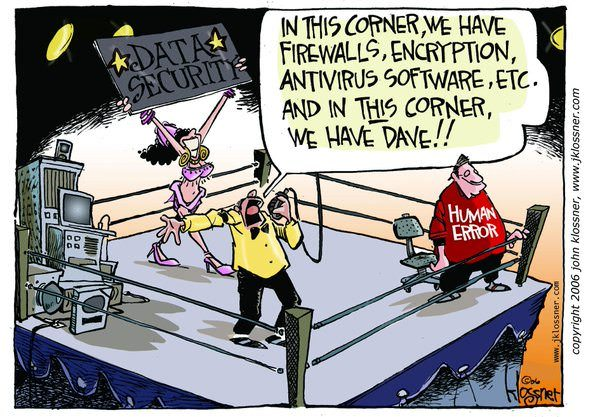
\includegraphics[width=.7\textwidth]{DaveSecurity}
\caption{Network Security - the sad truth}
\label{fig:dave}
\end{center}
\end{figure}

Note that, likewise tables and listings, you shall not worry about where the figures are placed. Moreover, you should not add the file extension (LaTeX will pick the `best' one for you) or the figure path.

%% !TEX root = ../Thesis.tex

\chapter{Conclusions and Future work}

They say that the conclusions are the shortened version of the introduction, and while the Introduction uses future verbs (we will), the conclusions use the past verbs (we did). It is basically true.

In the conclusions, you might also mention the shortcomings of the present work and outline what are the likely, necessary, extension of it.
E.g., we did analyse the performance of this network assuming that all the users are pedestrians, but it would be interesting to include in the study also the ones using bicycles or skateboards.

Finally, you are strongly encouraged to carefully spell check your text, also using automatic tools (like, e.g., Grammarly\footnote{\url{https://www.grammarly.com/}} for English language).

%--------------------------------------------------------------
% Bibliography
%--------------------------------------------------------------
%\bibliographystyle{unsrt} Entries are sorted by order of citation
\bibliographystyle{plain} 
\bibliography{Bibliography} % Entries are in the Bibliography.bib file

%--------------------------------------------------------------
\end{document}
%--------------------------------------------------------------
